\documentclass[a4paper,17pt]{extarticle}
\usepackage[utf8]{inputenc}
\usepackage{amsfonts}\usepackage{amssymb}\usepackage{amsmath}
\usepackage[top=2cm,left=1cm,right=1cm]{geometry}
\usepackage{tikz}
\usepackage{gensymb}\usepackage{ragged2e}\usepackage{blindtext}\usepackage{polynom} \usepackage{graphicx}



\begin{document}
\begin{center}
    MAT110 ASSIGNMENT 3 [SET-32]\\[6pt]
    NAME: ANIKA ISLAM \\[6pt]
    ID:21101298 \\[6pt]
    SECTION:08
\end{center}

\newpage
\begin{figure}[htbh!]
    \centering
    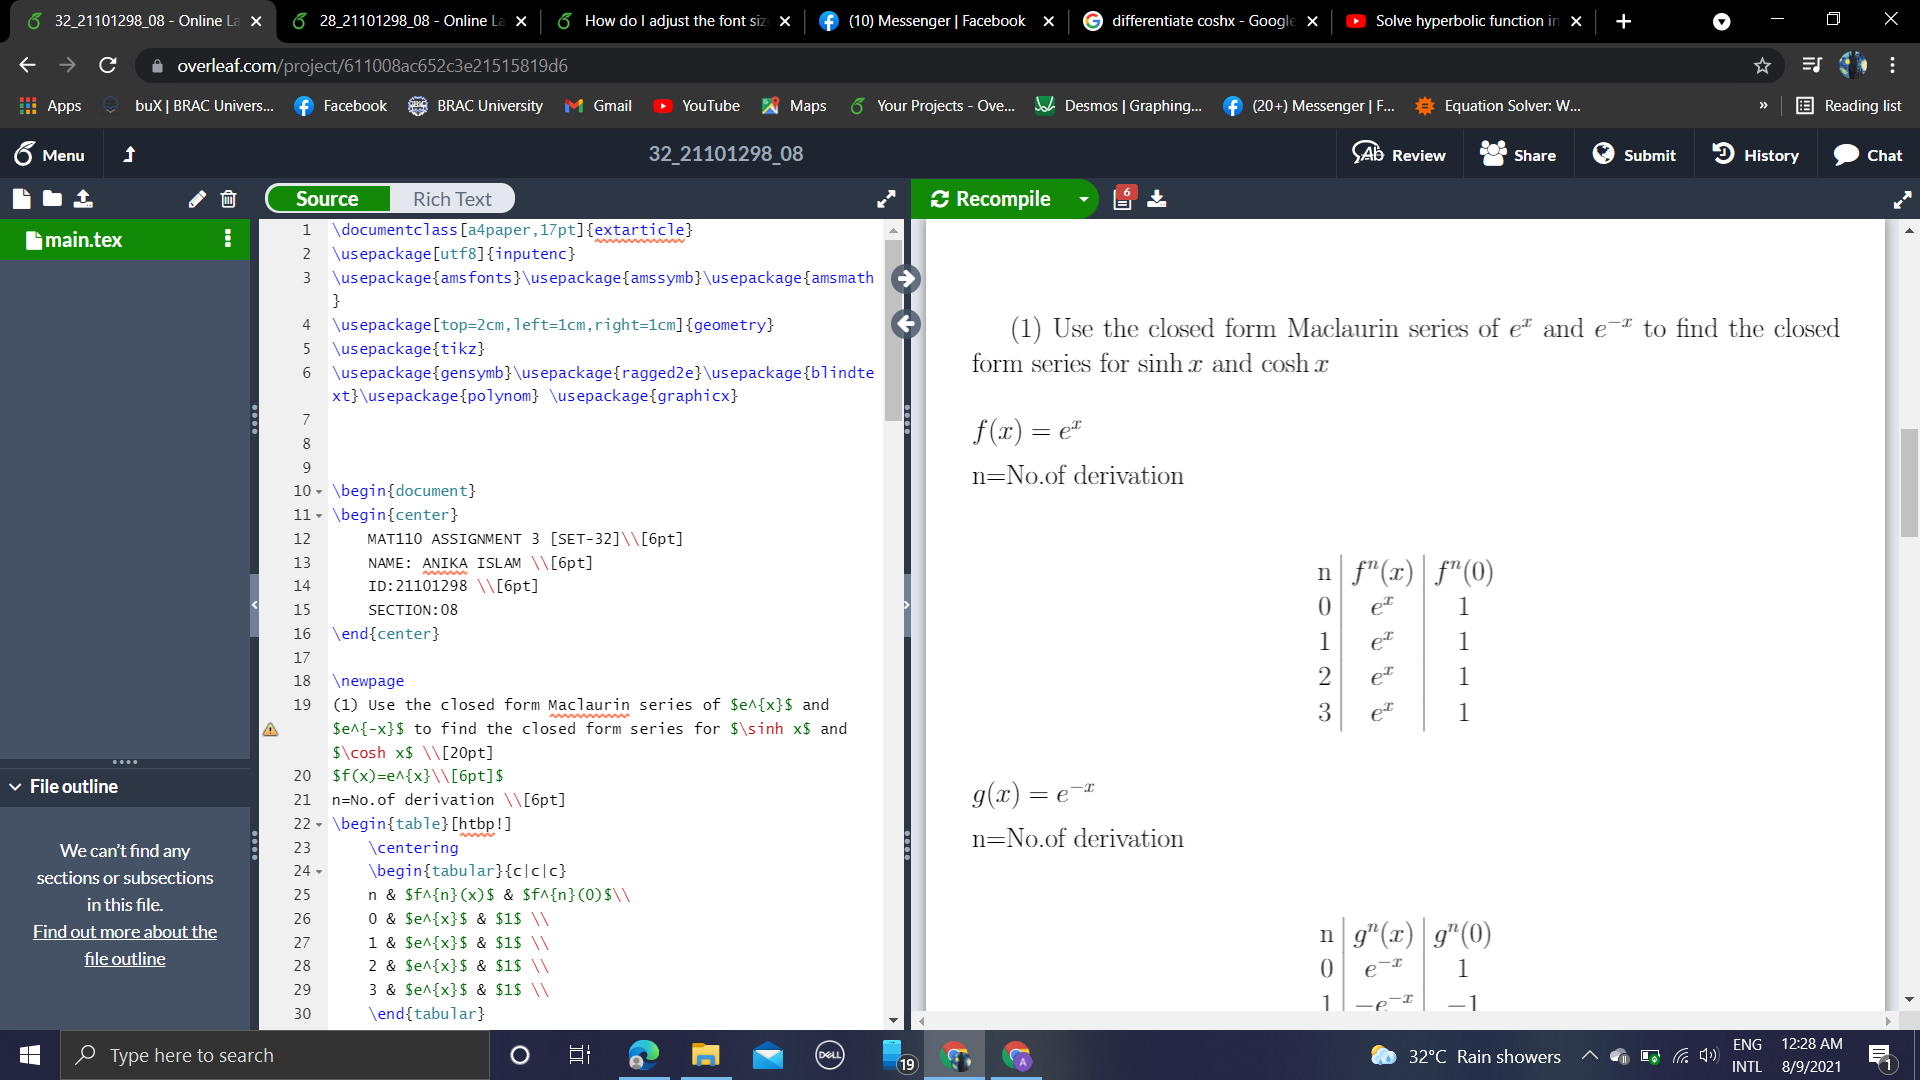
\includegraphics[width=1\linewidth]{SET 32.png}
    \caption{Screenshot of my Latex}
\end{figure}
\newpage
(1) Use the closed form Maclaurin series of $e^{x}$ and $e^{-x}$ to find the closed form series for $\sinh x$ and $\cosh x$ \\[20pt]
$f(x)=e^{x}\\[6pt]$
n=No.of derivation \\[6pt]
\begin{table}[htbp!]
    \centering
    \begin{tabular}{c|c|c}
    n & $f^{n}(x)$ & $f^{n}(0)$\\
    0 & $e^{x}$ & $1$ \\
    1 & $e^{x}$ & $1$ \\
    2 & $e^{x}$ & $1$ \\
    3 & $e^{x}$ & $1$ \\
    \end{tabular}
\end{table} \\[6pt]
$g(x)=e^{-x}\\[6pt]$
n=No.of derivation \\[6pt]
\begin{table}[htbp!]
    \centering
    \begin{tabular}{c|c|c}
    n & $g^{n}(x)$ & $g^{n}(0)$\\
    0 & $e^{-x}$ & $1$ \\
    1 & $-e^{-x}$ & $-1$ \\
    2 & $e^{-x}$ & $1$ \\
    3 & $-e^{-x}$ & $-1$ \\
    \end{tabular}
\end{table} \\[30pt]
$p(x)=\sinh x =\frac{f(x)-g(x)}{2}=\frac{e^{x}-e^{-x}}{2}\\[6pt]$
n=No.of derivation \\[6pt]
\begin{table}
    \centering
    \begin{tabular}{c|c|c}
    n & $p^{n}(x)$ & $p^{n}(0)$\\
    0 & $\sinh x = \frac{1}{2}(e^{x}-e^{-x})$ & $0$ \\
    1 & $\cosh x = \frac{1}{2}(e^{x}+e^{-x})$ & $1$ \\
    2 & $\sinh x = \frac{1}{2}(e^{x}-e^{-x})$ & $0$ \\
    3 & $\cosh x = \frac{1}{2}(e^{x}+e^{-x})$ & $1$ \\
    \end{tabular}
\end{table} \\[6pt]
\newpage
$\text{Using the closed form Maclaurin series of } \ e^{x} \  \text{and} \  e^{-x}, \\[6pt]
=>\sum_{n=0}^{\infty} \frac{p^{n}(0)x^{n}}{n!} = \frac{0}{0!}+\frac{1}{1!}x+\frac{0}{2!}x^{2}+\frac{1}{3!}x^{3}+....... \\[6pt]
= \frac{x}{1!}+\frac{x^{3}}{3!}+...... \\[6pt]
\sum_{n=0}^{\infty} \frac{x^{2n+1}}{2n!+1} \\[20pt]
q(x)=\sinh x =\frac{f(x)-g(x)}{2}=\frac{e^{x}-e^{-x}}{2}\\[6pt]$
n=No.of derivation \\[6pt]
\begin{table}[htbp!]
    \centering
    \begin{tabular}{c|c|c}
    n & $q^{n}(x)$ & $q^{n}(0)$\\
    0 & $\cosh x = \frac{1}{2}(e^{x}+e^{-x})$ & $1$ \\
    1 & $\sinh x = \frac{1}{2}(e^{x}-e^{-x})$ & $0$ \\
    2 & $\cosh x = \frac{1}{2}(e^{x}+e^{-x})$ & $1$ \\
    3 & $\sinh x = \frac{1}{2}(e^{x}-e^{-x})$ & $0$ \\
    4 & $\cosh x = \frac{1}{2}(e^{x}+e^{-x})$ & $1$ \
    \end{tabular}
\end{table} \\[6pt]
\newpage
$\text{Using the closed form Maclaurin series of } \ e^{x} \  \text{and} \  e^{-x}, \\[6pt]
=>\sum_{n=0}^{\infty} \frac{f^{n}(0)x^{n}}{n!} = \frac{1}{0!}+\frac{0}{1!}x+\frac{1}{2!}x^{2}+\frac{0}{3!}x^{3}+\frac{1}{4!}x^{4}+....... \\[6pt]
= 1+\frac{x^{2}}{2!}+\frac{x^{4}}{4!}+...... \\[6pt]
 \sum_{n=0}^{\infty} \  \frac{x^{2n}}{2n!} \\[20pt]$
%=======================================================
(2)Use Taylor series to evaluate
$$\lim_{x \to 0}=\frac{x^{3}-3x+3\arctan x}{x^{5}}$$\\[20pt]
$g(x)=\lim_{x \to 0}=\frac{x^{3}-3x+3\arctan x}{x^{5}}\\[6pt]
f(x)=x^{3}-3x \\[6pt]$
n=No.of derivation \\[6pt]
\begin{table}[htbp!]
    \centering
    \begin{tabular}{c|c|c}
    n & $f^{n}(x)$ & $f^{n}(0)$\\
    0 & $x^{3}-3x$ & $0$ \\
    1 & $3x^{2}-3$ & $-3$ \\
    2 & $6x$ & $0$ \\
    3 & $6$ & $6$ \\
    4 & $0$ & $0$ \\
    5 & $0$ & $0$ \
    \end{tabular}
\end{table} \\[6pt]
$y=\tan^{-1}x \\[6pt]
x=3\tan y \\[6pt]
\frac{dx}{dy}=3\sec^{2} y \\[6pt]
\frac{dy}{dx}=\frac{3}{sec^{2} y } \\[6pt]
\text{Using the equation} \ \sec^{2}y -\tan^{2}y =1 \\[6pt]
\sec^{2}y=1+x^{2} \\[6pt]
\frac{dx}{dy}=\frac{3}{(1+x^{2})}\\[6pt]
\frac{d^{2}x}{dy^{y}}=\frac{(1+x^{2})\frac{d}{dx}(3)-(3)\frac{d}{dx}{(1+x^{2})}}{(1+x^{2})^{2}}\\[6pt]
\frac{d^{2}}{dy^{2}}=\frac{0-3(2x)(1+x^{2})}{(1+x^{2})^{2}}\\[6pt]
\frac{d^{2}}{dy^{2}}=\frac{-6x}{(1+x^{2})^{2}}\\[6pt]
\frac{d^{3}}{dy^{3}}=\frac{(1+x^{2})^{2}\frac{d}{dx}(-6x)-(-6x)\frac{d}{dx}(1+x^{2})^{2}}{((1+x^{2})^{2})^{2}}\\[6pt]
\frac{d^{3}}{dy^{3}}=\frac{-6(1+x^{2})^{2}-(-6x)(2x)(2)(1+x^{2})}{(1+x^{2})^{4}}\\[6pt]
\frac{d^{3}}{dy^{3}}=\frac{-6(1-3x^{2})}{(1+x^{2})^{3}}\\[6pt]
\frac{d^{4}}{dy^{4}}=\frac{((1+x^{2})^{3})\frac{d}{dx}(-6+18x^{2})-(-6+18x^{2})\frac{d}{dx}((1+x^{2})^{3})}{((1+x^{2})^{3})^{2}}\\[6pt]
\frac{d^{4}}{dy^{4}}=\frac{((1+x^{2})^{3})(36x)-(-6+18x^{2})(3)(2x)((1+x^{2})^{2})}{((1+x^{2})^{6})}\\[6pt]
\frac{d^{4}}{dy^{4}}=\frac{72x(-x^{2}+1)}{(1+x^{2})^{4}}\\[6pt]
\frac{d^{5}}{dy^{5}}=\frac{((1+x^{2})^{4})\frac{d}{dx}(-72x^{3}+72x)-(-72x^{3}+72x)\frac{d}{dx}((1+x^{2})^{4})}{((1+x^{2})^{4})^{2}}\\[6pt]
\frac{d^{5}}{dy^{5}}=\frac{((1+x^{2})^{4})(-216x^{2}+72)-(-72x^{3}+72x)(4)(2x)((1+x^{2})^{3})}{((1+x^{2})^{8})}\\[6pt]
\frac{d^{5}}{dy^{5}}=\frac{72(5x^{4}-10x^{2}+1)}{((1+x^{2})^{8})}\\[6pt]$
\newpage
n=No. of derivative 
\begin{table}[htbp!]
    \centering
    \begin{tabular}{c|c|c}
        n & $y^{n}^(x)$ & $y^{n}(0)$ \\
        0 & $3\tan^{-1}x$ & $0$ \\
        1 & $\frac{3}{(1+x^{2})}$ & $3$ \\
        2 & $\frac{-6x}{(1+x^{2})^{2}}$ & $0$ \\
        3 & $\frac{-6(1-3x^{2})}{(1+x^{2})^{3}}$ & $-6$ \\
        4 & $\frac{72x(-x^{2}+1)}{(1+x^{2})^{4}}$ & $0$ \\
        5 & $\frac{72(5x^{4}-10x^{2}+1)}{((1+x^{2})^{8})}$ & $72$
    \end{tabular}
\end{table}\\[6pt]
Maclaurin series for f(x) = $ \frac{-3x}{1!}+\frac{6x^{3}}{3!} = -3x+x^{3} \\[6pt]
\text{Maclaurin series for y} = \frac{3x}{1!}-\frac{6x^{3}}{3!}+\frac{72x^{5}}{5!} = 3x-x^{3}+\frac{3x^{5}}{5}\\[6pt]
\text{Maclaurin series for  g(x)} = \frac{ -3x + x^{3} +3x - x^{3} +\frac{3x^{5}}{5}}{x^{5}}\\[6pt]
=\frac{\frac{3x^{5}}{5}}{x^{5}} \\[6pt]
=\frac{3}{5} \\[20pt]$
%=======================================================
(3)$f(x)=\begin{cases}
e^{\frac{-1}{x^{2}}} \ , \ x \not = 0 \\
0 \ , \ x=0\\
\end{cases}$\\[6pt]
Show that f(x) is not equal to its Maclaurin series \\[20pt]
$f(x)=e^{\frac{-1}{x^{2}}} \\[6pt]
\text{At} \ f(x) = e^{\frac{-1}{(0)^{2}}} = \infty \   \\[6pt]
f'(x) = -(\frac{0-2x}{x^{4}})e^{\frac{-1}{x^{2}}}\\[6pt]
f'(x) = \frac{2e^{\frac{-1}{x^{2}}}}{x^{3}} \\[6pt]
\text{At} \ f'(x) = \frac{0}{0} \  \text{(Intermediate form)} \\[6pt]
\text{Using L'Hopital Rule} \\[6pt]
=\frac{2}{x^{3}e^{\frac{1}{x^{2}}}}........(\text{Multiplying by} \ x^{3}) \\[6pt]
=\frac{\frac{2}{x^{3}}}{e^{\frac{1}{x^{2}}}}\\[6pt]
=\frac{\frac{2(-3)}{x^{4}}}{\frac{2e^{\frac{-1}{x^{2}}}}{x^{3}}}\\[6pt]
=\frac{-3}{xe^{\frac{1}{x^{2}}}}\\[6pt]
\text{At} \ x=0, \\[6pt]
=\frac{-3}{(0)e^{\frac{1}{x^{2}}}}\\[6pt]
=\frac{-3}{\infty}\\[6pt]
=0\\[6pt]
\text{Maclaurin series:} \ \frac{0}{1!}x+.........\\[6pt]
=0+.....\\[6pt]
\text{At} \ x=0, f(x) \ \text{does not have a finite value, whereas, in the Maclaurin series ,}\\[2pt]
\text{there is a finite value,therefore,} \ f(x) \not = \text{Maclaurin series} \\[20pt]$
%======================================================
(4)Let 
$$f(x)=\begin{cases}
\frac{x^{3}y - xy^{3}}{x^{2}+y^{2}} \ , \ x \not = 0 \\
0 \ , \ x=0\\
\end{cases}\\
$$\\[6pt]
Find $f_{x}(0,0)$ \ and $f_{y}(0,0)$\\[20pt]
For $f_{x}(0,0) => \lim_{\Delta x \to 0} \  \frac{f(x+\Delta x,y)-f(x,y)}{\Delta x} \\[6pt]
=> \lim_{\Delta x \to 0} \ \frac{f(0+\Delta x,0)-f(0,0)}{\Delta x}\\[6pt]
=> \lim_{\Delta x \to 0} \ \frac{ \frac{\Delta x^{3}(0)- \Delta x(0)^{3}}{\Delta x^{2}+(0)^{2}}}{\Delta x}\\[6pt]
=> \lim_{\Delta x \to 0} \ \frac{0}{\Delta x^{3}}\\[6pt]
\therefore f_{x}(0,0)=0\\[6pt]
f_{y}(0,0) => \lim_{\Delta y \to 0} \  \frac{f(x ,y+\Delta y)-f(x,y)}{\Delta y} \\[6pt]
=> \lim_{\Delta y \to 0} \ \frac{f(x,0+\Delta y)-f(0,0)}{\Delta y}\\[6pt]
=> \lim_{\Delta y \to 0} \ \frac{ \frac{(0)^{3}(\Delta y)- (0)(\Delta y)^{3}}{(0)^{2}+(\Delta y)^{2}}}{\Delta y}\\[6pt]
=> \lim_{\Delta y \to 0} \ \frac{0}{\Delta y^{3}} \\[6pt]
\therefore f_{y}(0,0)=0\\[20pt]$
%=========================================================
(5)If $z=f(x,y)$ where $x=r\cos \theta$ and $y=r\sin \theta$,find $\frac{\partial z}{\partial r}, \frac{\partial r}{\partial \theta},\frac{\partial^{2}z}{\partial r \partial \theta} $ \\[20pt]
$\frac{\partial f(x,y)}{\partial x} = f_{x} \\[6pt]
\frac{\partial f(x,y)}{\partial y} = f_{y} \\[6pt]
\frac{\partial x }{\partial \theta} = -r\sin \theta \\[6pt]
\frac{\partial x}{\partial r} = \cos \theta \\[6pt]
\frac{\partial y}{\partial \theta} = r\cos \theta \\[6pt]
\frac{\partial y}{\partial r} = \sin \theta \\[6pt]
\text{for} \ \frac{\partial z}{\partial r}:\\[6pt]
=>\frac{\partial z}{\partial r} = \frac{\partial z}{\partial x}.\frac{\partial x}{\partial r} + \frac{\partial z}{\partial y}.\frac{\partial y}{\partial r}\\[6pt]
=>\frac{\partial z}{\partial r}=f_{x}\cos \theta + f_{y} \sin \theta \\[6pt]
\text{for} \ \frac{\partial z}{\partial \theta}:\\[6pt]
=>\frac{\partial z}{\partial \theta} = \frac{\partial z}{\partial x}.\frac{\partial x}{\partial \theta} + \frac{\partial z}{\partial y}.\frac{\partial y}{\partial \theta}\\[6pt]
=>\frac{\partial z}{\partial \theta}=f_{x}(-r\sin \theta) + f_{y}( r\cos \theta )\\[6pt]
=>\frac{\partial z}{\partial \theta}=r(-f_{x}\sin \theta + f_{y}\cos \theta )\\[6pt]$
\newpage
$\text{for} \ \frac{\partial^{2} z}{\partial r \partial \theta}:\\[6pt]
=>\frac{\partial^{2} z}{\partial r \partial \theta}=
-f_{xx}\sin \theta + f_{yy} \cos \theta\\[20pt]$
%===========================================================
(6)A manufacturer has modeled its yearly production function P (the value
of its entire production, in millions of dollars) as a Cobb-Douglas function
$P(L, K) = 1.47L^{0.65}K^{0.35}$ where L is the number of labor hours (in thousands) and K is the invested capital (in millions of dollars). Suppose that
when L = 30 and K = 8, the labor force is decreasing at a rate of $2000$ labor
hours per year and capital is increasing at a rate of $\$500,000$ per year. Find
the rate of change of production.\\[20pt]
$P(L, K) = 1.47L^{0.65}K^{0.35}\\[6pt]
P(L, K) = 1.47(30)^{0.65}(8)^{0.35}\\[6pt]
P(L, K)=27.77\\[6pt]
P=1.47L^{0.65}K^{0.35}\\[6pt]
=> \ln P(L,K) = \ln1.47  + 0.65\ln L +0.35\ln K \\[6pt]
\text{for} \ \frac{\partial P}{\partial L}:\\[6pt]
=> \frac{1}{P}\frac{\partial P}{\partial L} = 0+ \frac{0.65}{L}\\[6pt]
=> \frac{\partial P}{\partial L} = P(\frac{0.65}{L}) \\[6pt]
=> \frac{\partial P}{\partial L} = (27.77)(\frac{0.65}{30}) \\[6pt]
=> \frac{\partial P}{\partial L} =0.601\\[20pt]
\text{for} \ \frac{\partial P}{\partial K}:\\[6pt]
=> \frac{1}{P}\frac{\partial P}{\partial K} =0+\frac{0.35}{K} \\[6pt]
=> \frac{\partial P}{\partial K} = P(\frac{0.35}{K}) \\[6pt]
=> \frac{\partial P}{\partial K} = (27.77)(\frac{0.35}{8}) \\[6pt]
=> \frac{\partial P}{\partial K} =1.21\\[20pt]
\text{Given} \ \frac{\partial L }{\partial t} = 2000 \ \text{and} \ \frac{\partial K}{\partial t} = 500,000 \\[6pt]
\text{for} \ \frac{\partial P}{\partial t} :\\[6pt]
=>\frac{\partial P}{\partial t}=\frac{\partial P}{\partial L}.\frac{\partial L}{\partial t} + \frac{\partial P}{\partial K}.\frac{\partial K}{\partial t}\\[6pt]
=>\frac{\partial P}{\partial t}=(0.601)(2000)+(1.21)(500000)\\[6pt]
=>\frac{\partial P}{\partial t}= \$606202  \ \text{per year}$
%=========================================================
\end{document}
